\section{Single-Day Validation Results}
\label{sec:single_day}

Before extending to multi-day regimes, we establish that LLMs can detect single-day dealer constraints under obfuscation---a prerequisite for temporal regime identification. This section summarizes results from our companion single-day study \citep{regan2025obfuscation} and presents the raw chain validation that motivates the regime detection extension.

\subsection{Detection Under Obfuscation}

Applied to 242 trading days (SPY, 2024), the obfuscation framework achieved 71.5\% detection of dealer hedging patterns using unbiased prompts, with 91.2\% predictive accuracy on forward returns. The WHO$\rightarrow$WHOM$\rightarrow$WHAT causal framework achieved $>$90\% correct specification across all three components, confirming the model articulates mechanical reasoning rather than pattern labels.

Detection remained stable across quarters: 68.2\% (Q1), 70.5\% (Q2), 72.8\% (Q3), and 73.6\% (Q4), with no statistically significant seasonal variation ($p = 0.84$). This temporal stability is critical---it confirms the framework identifies structural properties rather than period-specific memorization.

\subsection{Raw Chain Validation}
\label{subsec:raw_chain}

A key finding with direct implications for financial AI pipeline design: when provided raw strike-level options chain data (without pre-calculated GEX metrics), the LLM achieved 92.3\% detection---outperforming the GEX-assisted baseline of 61.5\% by 30.8 percentage points (Table~\ref{tab:raw_chain}).

\begin{table}[H]
\centering
\caption{Raw chain vs.\ GEX-assisted detection on 13 identical test dates. Raw strike-level data substantially outperforms pre-calculated parametric summaries. Reasoning quality assessed across all raw chain responses ($n = 13$).}
\label{tab:raw_chain}
\begin{tabular}{@{}lr@{}}
\toprule
\textbf{Metric} & \textbf{Result} \\
\midrule
\multicolumn{2}{@{}l}{\textit{Detection comparison}} \\
Raw Chain Detection Rate & 92.3\% (12/13) \\
GEX-Assisted Baseline & 61.5\% (8/13) \\
Improvement & +30.8 pp \\
\midrule
\multicolumn{2}{@{}l}{\textit{Reasoning quality (raw chain, $n = 13$)}} \\
Identifies market makers (WHO) & 100\% (13/13) \\
Identifies counterparties (WHOM) & 84.6\% (11/13) \\
Explains hedging mechanism (WHAT) & 100\% (13/13) \\
Avg reasoning score & 5.5/6 \\
\bottomrule
\end{tabular}
\end{table}

This result establishes that parametric GEX represents \textit{lossy compression} of structural signal: the scalar aggregation discards strike-level distribution information that enables the model to identify dealer positioning with higher fidelity. The finding has practical implications for financial data pipeline design---providing LLMs with raw, structured data rather than pre-processed summaries may yield superior analytical performance across domains.

\subsection{Detection-Alpha Orthogonality}

A critical validation that the framework detects structural mechanisms rather than profit opportunities: detection rates remained stable (68--74\% quarterly) while a naive trading strategy based on detections saw its Sharpe ratio collapse from 1.8 (Q1) to 0.1 (Q4). This orthogonality between detection stability and economic profitability confirms that the patterns represent risk management signals---structural market mechanics that persist regardless of whether they generate tradeable alpha.

\subsection{Inverse P-Hacking Defense}

To address concerns about specification searching, we conducted an inverse p-hacking analysis: comparing outcome metrics on 519 detection days against a 100-day random baseline of non-detection days. If the framework were p-hacking---selecting days that happen to show dramatic market moves---detected days should exhibit \textit{higher} realized volatility and range expansion than random. Instead, detected days showed 33\% \textit{lower} range expansion than the baseline (lift = 0.67$\times$, $\chi^2 = 4.53$, $p = 0.033$). This inverse relationship confirms the framework detects dampening mechanisms (dealer hedging that suppresses volatility) rather than amplifying events---a result that cannot arise from specification searching.



\section{Regime Detection and Market Evolution}
\label{sec:regime}

Building on single-day validation, we extend to 30-day persistent regime detection across five phases spanning 2020--2025.

\paragraph{Statistical conventions used in this section.}
Detection rates are reported as point estimate followed by a 95\%
confidence interval in brackets. For phases where per-window records
are available (Phases 1--4 and Phase 2 negative controls), the CI is
a 10{,}000-replicate percentile bootstrap over windows; for the Phase 5
per-year rates where only aggregate counts are retained in the published
results, we report the equivalent 95\% Wilson score interval, which has
the same coverage properties for binomial proportions and is standard in
clinical and survey statistics \citep{brown2001interval}. All CIs are
produced deterministically by
\texttt{scripts/validation/paper2/jrfm\_revision/bootstrap\_detection\_ci.py}
in the accompanying code release.

Figure~\ref{fig:validation_pipeline} summarizes detection rates across all validation phases.

\begin{figure}[H]
\centering
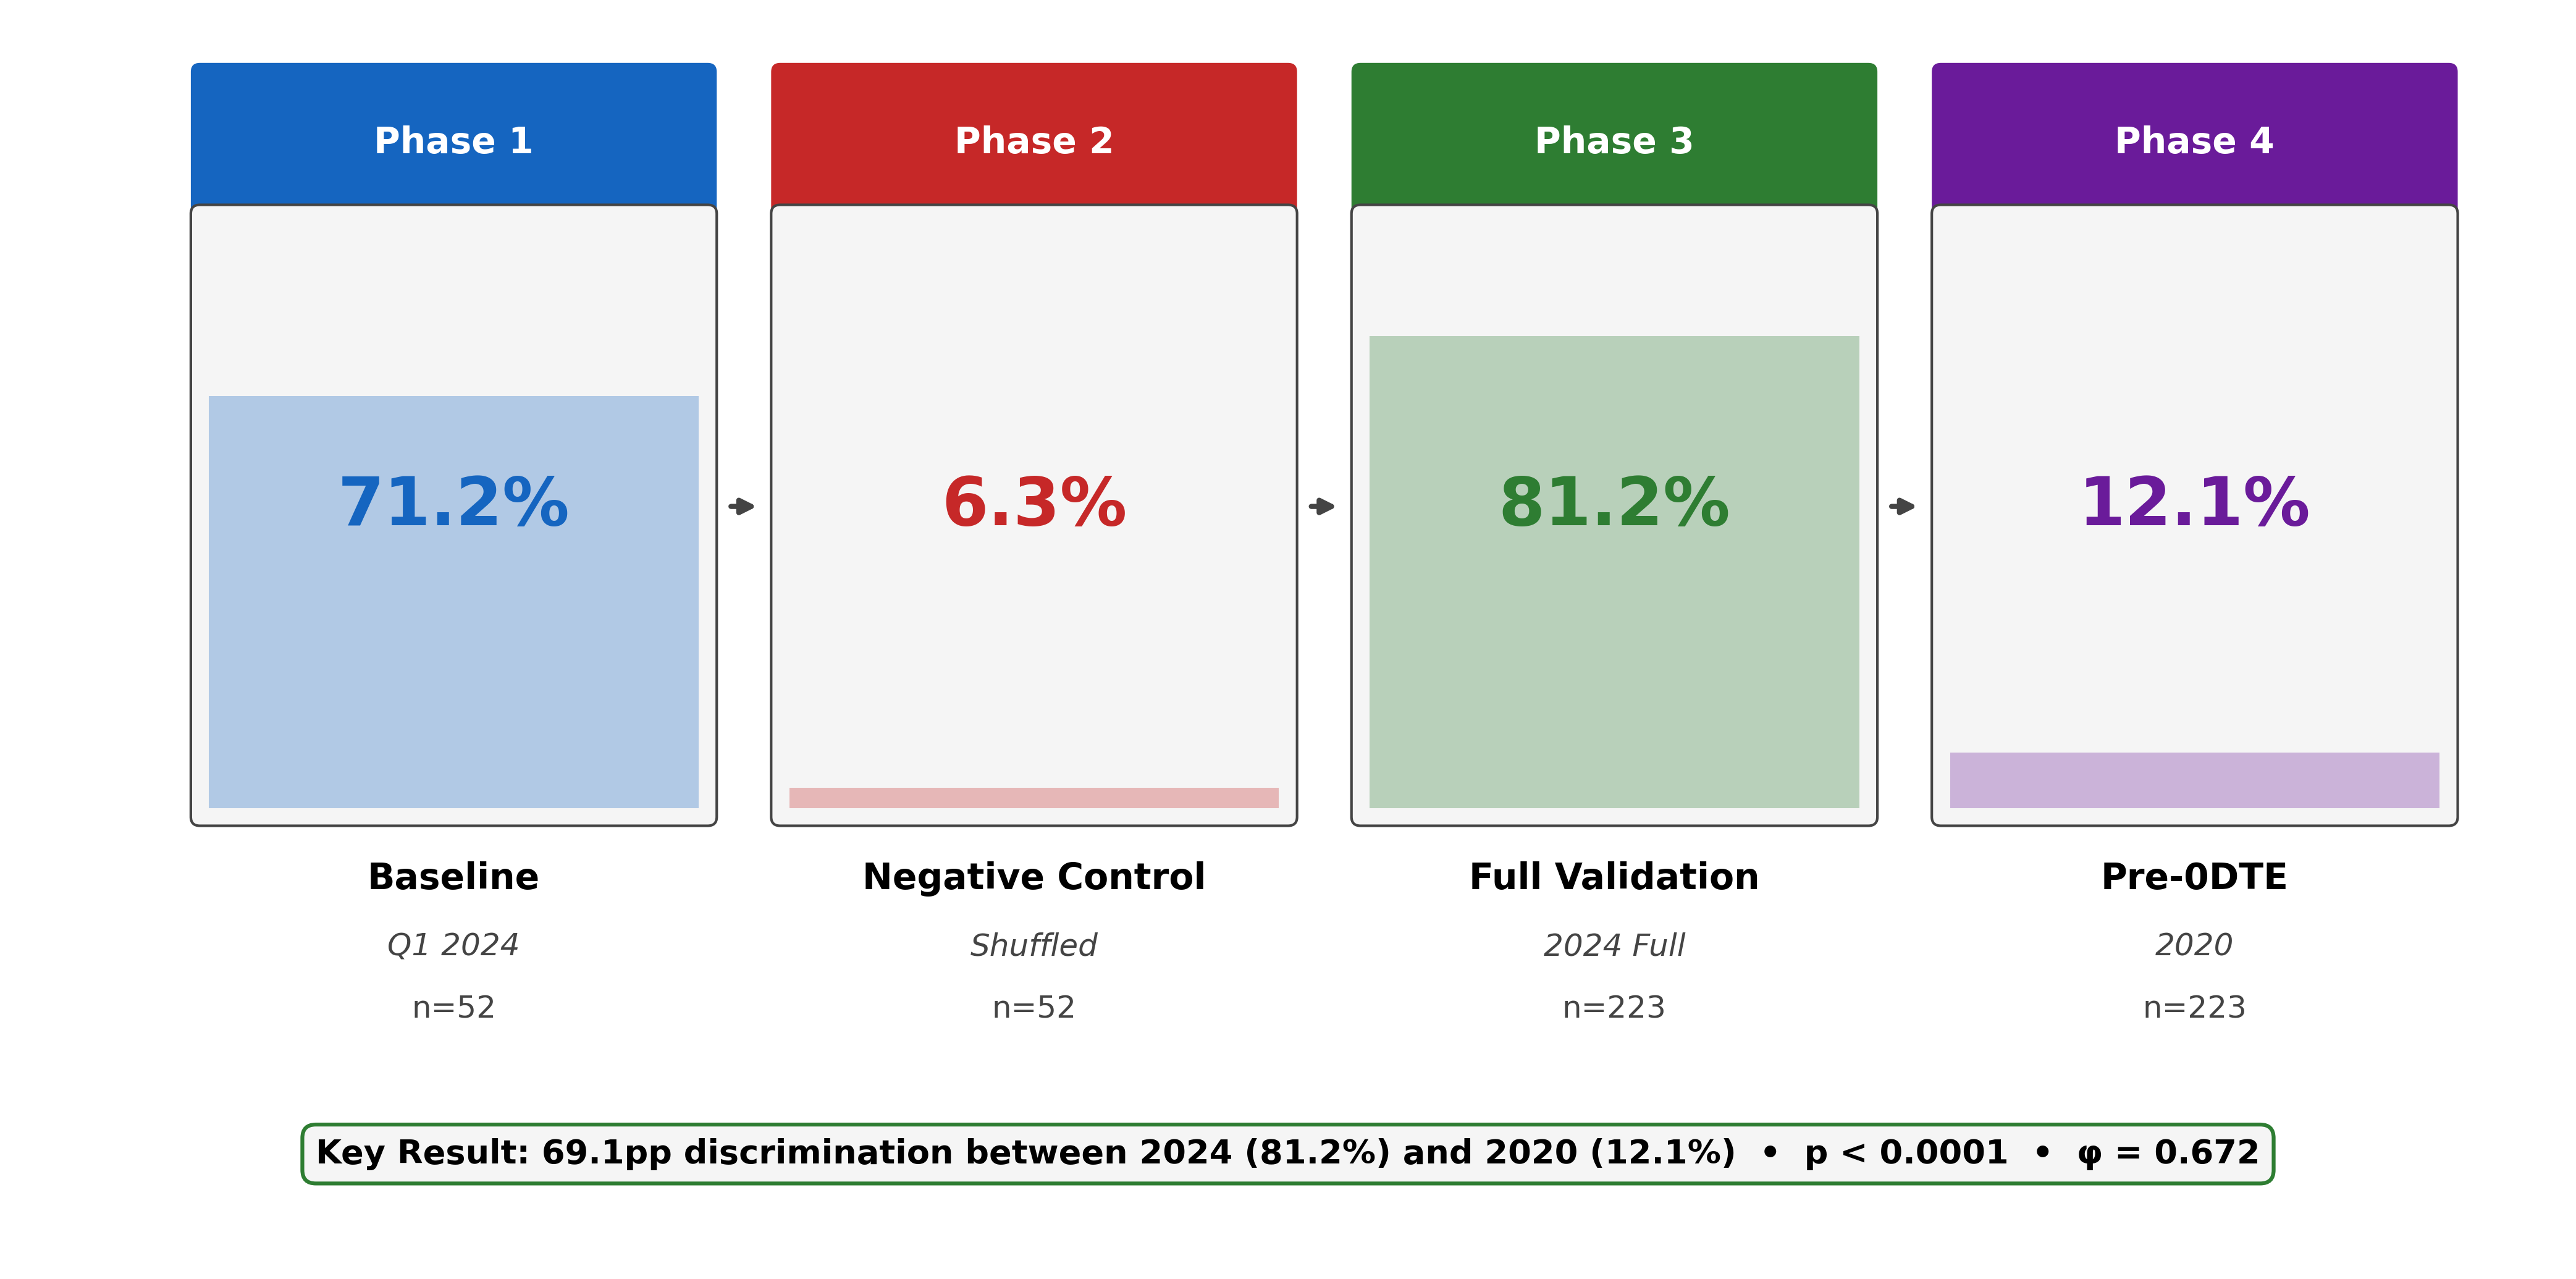
\includegraphics[width=\textwidth]{figures/fig03_validation_pipeline.png}
\caption{Multi-phase validation pipeline. Each box reports the phase name, the number of 30-day windows evaluated, and the detection rate with 95\% bootstrap confidence interval. Phase~1 (Q1 2024 baseline) anchors the framework at 71.2\% detection; Phase~2 synthetic controls (shuffle/transitional/low-magnitude) test false-positive discipline; Phase~3 (full 2024) confirms 81.2\% generalisation; Phase~4 (full 2020) is the pre-0DTE baseline at 12.1\%; Phase~5 extends to a 2020--2025 panel. \textbf{Read this figure as:} the phase-by-phase progression from narrow baseline to full multi-year panel, with rate separation preserved at every stage.}
\label{fig:validation_pipeline}
\end{figure}

\subsection{Phase 1--3: Baseline and Full-Year Validation}

Phase 1 established a 71.2\% detection rate on Q1 2024 (37/52 windows; 95\% CI [57.7, 82.7]\%), with strong discrimination: detected windows averaged 95.8\% persistence versus 58.0\% for rejected windows (+37.8 pp gap), and \$13.1B versus \$5.9B magnitude (+\$7.2B gap). Phase 3 extended to full 2024 (223 windows), finding 81.2\% detection (181/223; 95\% CI [75.8, 86.1]\%)---100\% persistent negative regimes with no false classifications on regime type. The framework correctly rejected 42 windows (18.8\%) exhibiting February--March volatility (6--10 sign flips).

\subsection{Phase 2: Negative Controls}

Phase 2 validated framework discrimination through three synthetic tests (Table~\ref{tab:negative_controls}).

\begin{table}[H]
\centering
\caption{Phase 2 negative control results (false positive rates with 95\% bootstrap CIs; Wilson upper bounds shown in square brackets for the zero-detection rows, where bootstrap intervals degenerate to zero). Transitional and low-magnitude controls achieve statistically reliable discrimination.}
\label{tab:negative_controls}
\begin{tabular}{@{}lrrr@{}}
\toprule
\textbf{Test} & \textbf{2024 FP (95\% CI)} & \textbf{2020 FP (95\% CI)} & \textbf{Criterion} \\
\midrule
Shuffle & 61.1\% [48.1, 74.1]\% (33/54) & 12.1\% [8.1, 16.6]\% (27/223) & diagnostic \\
Transitional & 0.0\% [0.0, 10.7]\% (0/32) & 0.0\% [0.0, 1.7]\% (0/223) & $<$10\% \\
Low-Magnitude & 0.0\% [0.0, 6.6]\% (0/54) & 0.0\% [0.0, 1.7]\% (0/223) & $<$10\% \\
\bottomrule
\end{tabular}
\end{table}

Transitional and low-magnitude tests achieved perfect 0\% false positive rates, confirming the framework enforces all three regime criteria simultaneously. The shuffle test revealed regime-dependent behavior: 2020 shuffled data passed (12.1\% FP), while 2024 shuffled data exceeded the criterion (61.1\% FP). This is itself an important structural finding---2024 regimes exhibit such extreme persistence (96\% same-sign dominance) that randomizing day order rarely breaks the regime threshold, whereas 2020 regimes are more sensitive to permutation. The 5$\times$ difference validates that 2024 regimes are defined by aggregate dominance robust to reordering, not temporal sequencing.

\subsection{Phase 4: 2020 vs.\ 2024 Comparison}

Phase 4 revealed a 69.1 percentage point detection difference between eras (Table~\ref{tab:phase4}).

\begin{table}[H]
\centering
\caption{Phase 4: 2020 vs.\ 2024 market structure comparison. The large effect size ($\varphi = 0.69$) confirms fundamentally different market structures; full test statistics in-text below the table.}
\label{tab:phase4}
\begin{tabular}{lrrr}
\toprule
\textbf{Metric} & \textbf{2024} & \textbf{2020} & \textbf{Difference} \\
\midrule
Detection Rate & 81.2\% [75.8, 86.1]\% (181/223) & 12.1\% [8.1, 16.6]\% (27/223) & +69.1 pp \\
Avg Persistence (detected) & 98.2\% & 100.0\% & $-$1.8 pp \\
Avg Magnitude (detected) & \$30.5B & \$5.5B & +\$25.0B \\
Avg Magnitude (rejected) & \$31.8B & \$2.2B & +\$29.6B \\
Dominant Sign & Negative & Positive & Flip \\
0DTE Volume Share (SPY) & $\approx$46\% & $<$5\% & -- \\
\bottomrule
\end{tabular}
\end{table}

The 2020 baseline (12.1\% detection) confirms framework selectivity: dealer gamma hedging was active but at lower magnitude (\$2.2B average for rejected windows vs.\ \$5.5B for the 27 detected), and 87.9\% of windows failed regime criteria. Notably, 2024 rejected windows had \textit{higher} average magnitude (\$31.8B) than detected windows (\$30.5B), confirming that rejection is driven by stability (sign flips), not magnitude---consistent with the February--March volatility noted in Phase 3. The separation between the two eras is statistically overwhelming:
Pearson's $\chi^2 = 213.67$ (df $= 1$, $p = 2.2 \times 10^{-48}$; Yates-corrected $\chi^2 = 210.90$, $p = 8.7 \times 10^{-48}$),
Fisher's exact test gives a two-sided $p = 1.8 \times 10^{-52}$ with odds ratio 31.3 (detected-vs-not odds for 2024 are 31-fold higher than for 2020),
the phi coefficient $\varphi = 0.69$ indicates a large effect by Cohen's convention,
and the risk difference is 69.1 percentage points (95\% Wald CI [62.4, 75.7]~pp).
Together these statistics confirm fundamentally different market structures between pre-0DTE and post-0DTE eras, not a marginal shift.

\begin{figure}[H]
\centering
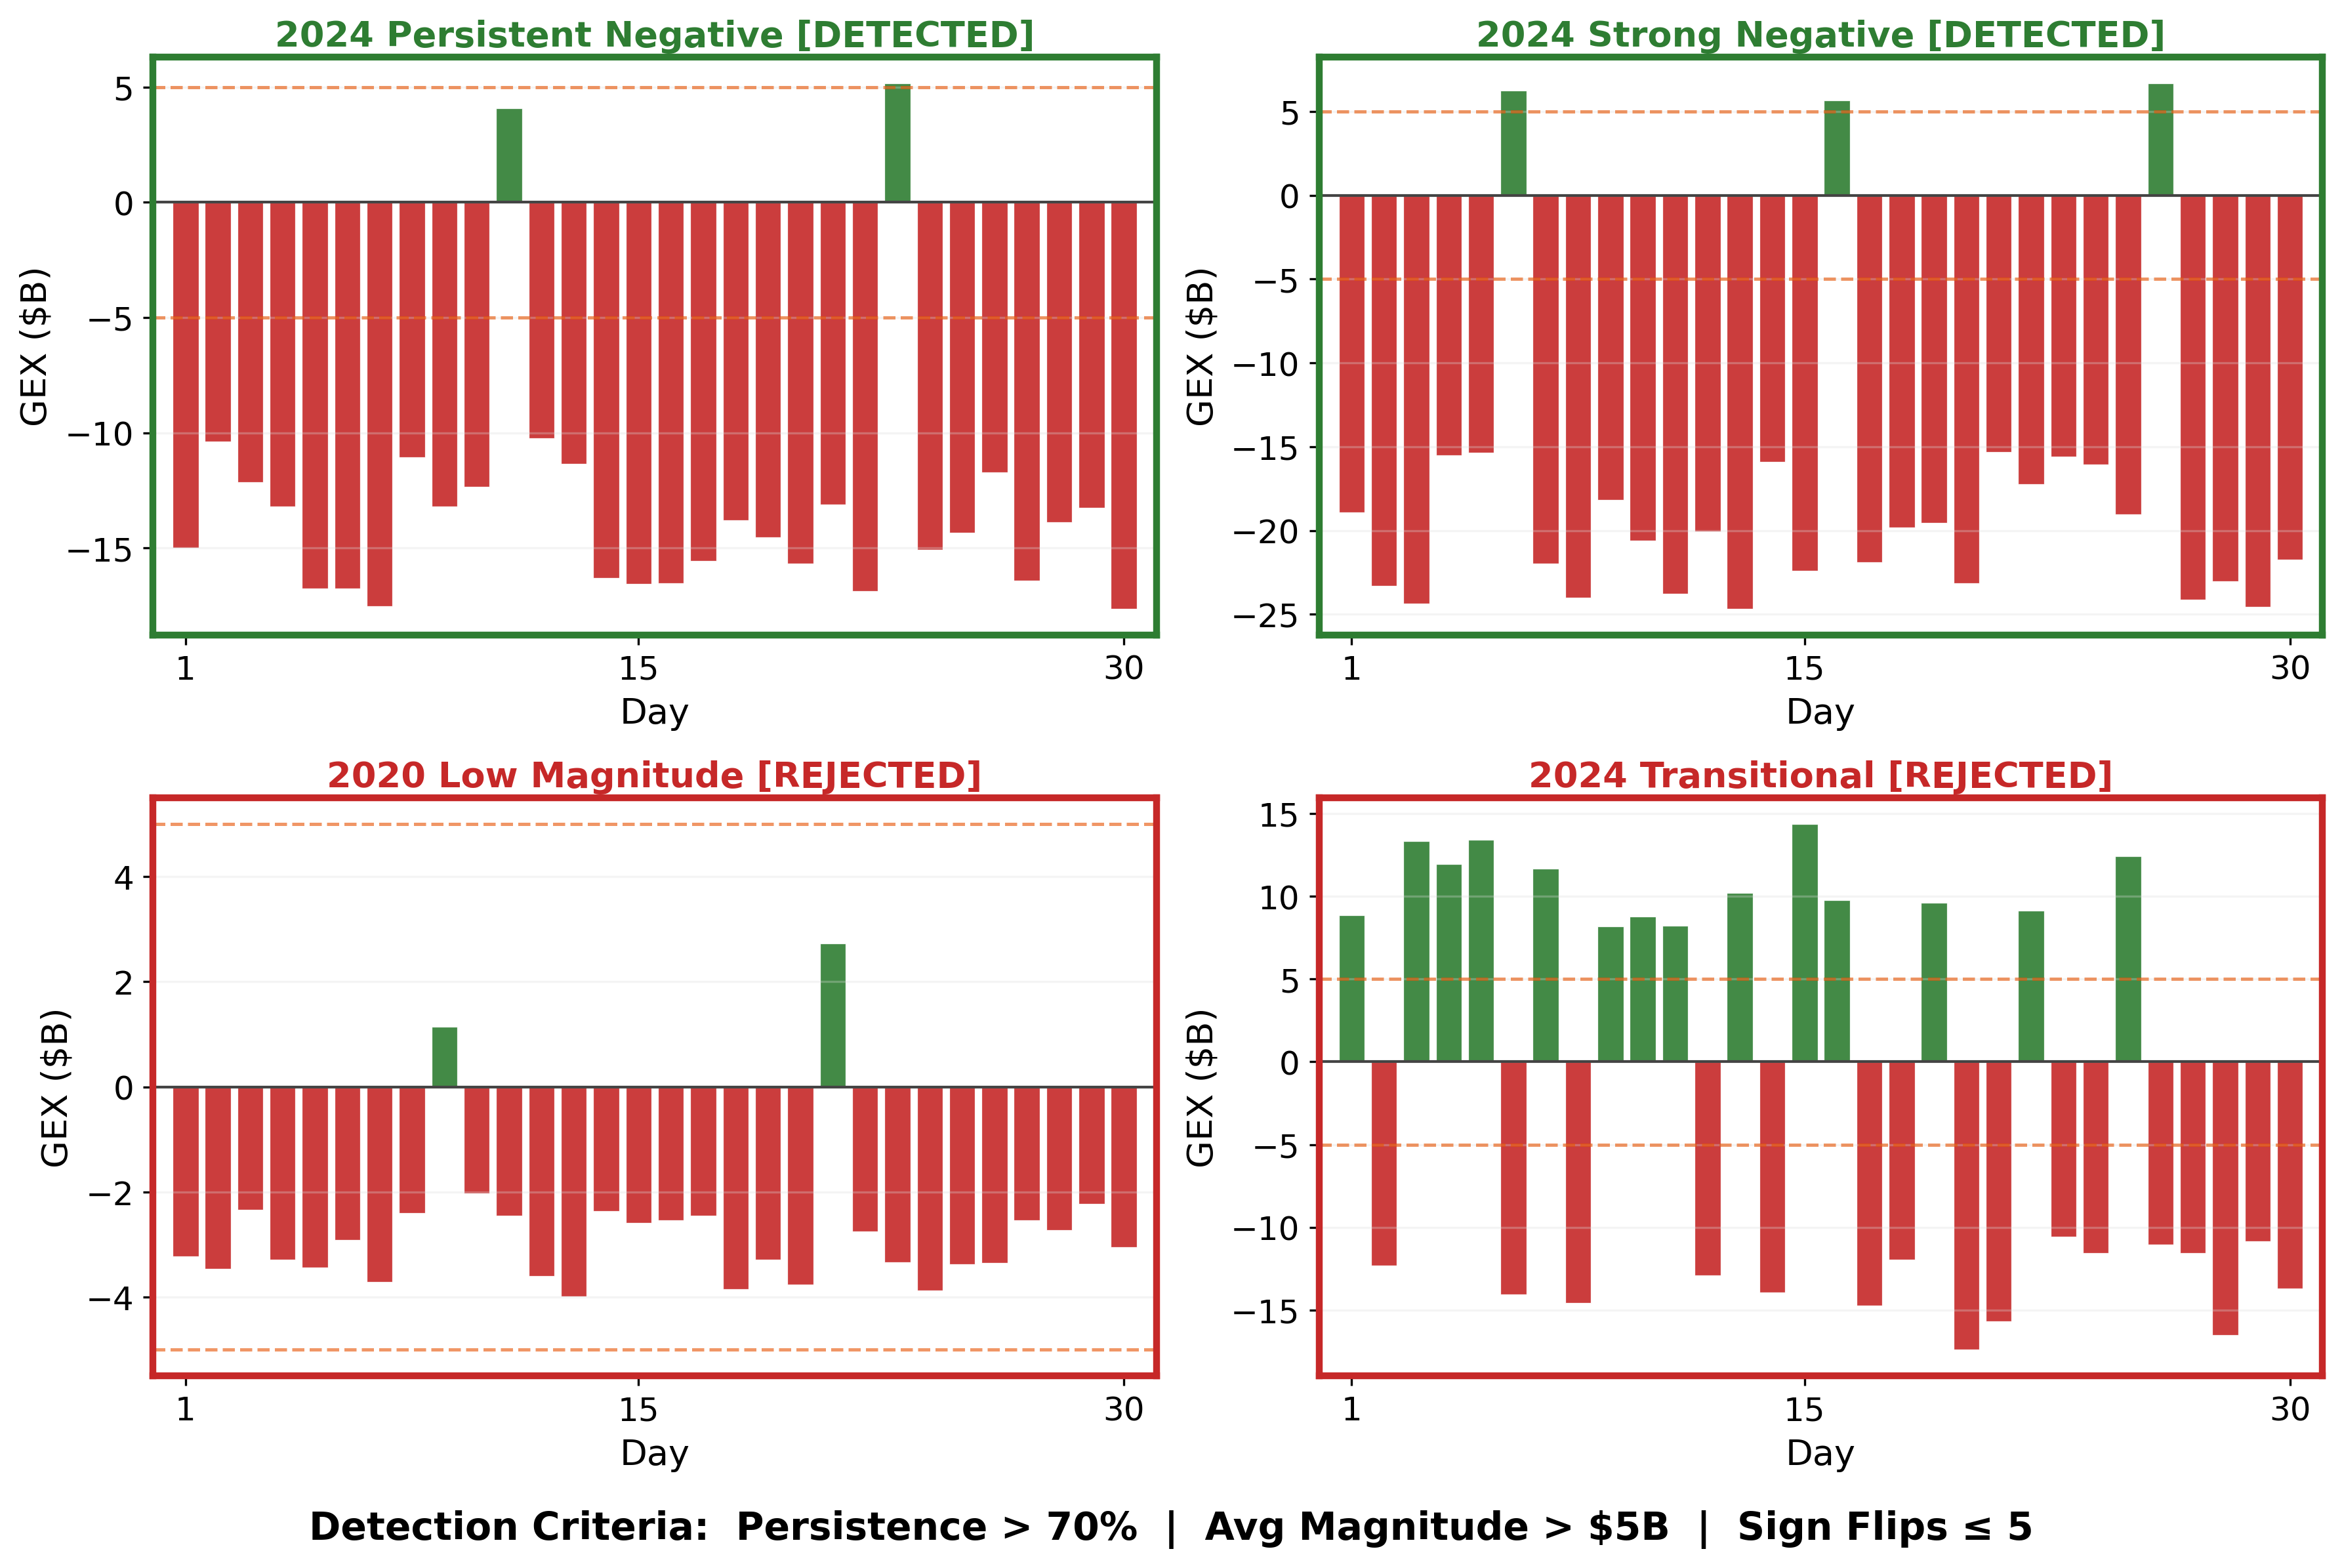
\includegraphics[width=\textwidth]{figures/fig04_selectivity.png}
\caption{Framework selectivity illustrated on four example 30-day windows. \textbf{Top row (detected):} a 2024-Q2 persistent negative regime (28/30 days negative, \$30B average magnitude, 3 sign flips) and a 2024-Q4 persistent negative regime (27/30, \$25B, 2 flips); both meet all three criteria. \textbf{Bottom row (rejected):} a February 2024 window rejected for stability (only 55\% persistence with 8 sign flips despite high magnitude) and a 2020-Q2 window rejected for magnitude (90\% persistence but only \$2.8B average). \textbf{Read this figure as:} detection is not a function of a single criterion but of all three acting jointly --- high magnitude alone or high persistence alone is not sufficient.}
\label{fig:selectivity}
\end{figure}

\subsection{Phase 5: Multi-Year Temporal Evolution (2020--2025)}

Phase 5 extended analysis to 1,412 windows across six years, revealing gradual regime evolution rather than sharp transition (Table~\ref{tab:phase5}).

\begin{table}[H]
\centering
\caption{Phase 5: Multi-year detection rates with 95\% Wilson score confidence intervals (2020--2025). The 2020 and 2024--2025 CIs do not overlap, supporting the structural-shift interpretation. Detection tracks 0DTE adoption with a tipping point at 2024.}
\label{tab:phase5}
\footnotesize
\begin{tabular}{@{}lrrrlrl@{}}
\toprule
\textbf{Year} & \textbf{Win.} & \textbf{Det.} & \textbf{Rate} & \textbf{95\% CI} & \textbf{Avg GEX} & \textbf{Status} \\
\midrule
2020 & 213 & 26 & 12.2\% & [8.5, 17.3]\% & \$3.0B & Pre-regime \\
2021 & 241 & 9 & 3.7\% & [2.0, 6.9]\% & \$4.9B & Borderline \\
2022 & 244 & 79 & 32.4\% & [26.8, 38.5]\% & \$5.5B & Growing \\
2023 & 228 & 46 & 20.2\% & [15.5, 25.9]\% & \$9.6B & Inconsistent \\
2024 & 241 & 241 & 100\% & [98.4, 100.0]\% & \$20.3B & Structural shift \\
2025 & 245 & 245 & 100\% & [98.5, 100.0]\% & \$19.0B & Sustained \\
\midrule
\textbf{Total} & \textbf{1,412} & \textbf{646} & \textbf{45.8\%} & \textbf{[43.2, 48.4]\%} & \textbf{--} & \textbf{--} \\
\bottomrule
\end{tabular}
\end{table}

Detection rates track 0DTE market penetration (3.7\% in 2021 $\rightarrow$ 100\% in 2024), with average GEX magnitude growing from \$3.0B (2020) to \$20.3B (2024)---a roughly 577\% increase far exceeding cumulative inflation. The 2023$\rightarrow$2024 transition is statistically unambiguous: Pearson's $\chi^2 = 314.4$ ($\text{df} = 1$, $p = 2.4 \times 10^{-70}$), Fisher's exact $p = 9.9 \times 10^{-87}$ (odds ratio diverges because all 241 windows in 2024 are detected), and $\varphi = 0.82$. This marks a structural reorganization of dealer positioning rather than a gradual drift. Sustained 100\% detection through 2024--2025 (486/486 windows) suggests stable post-0DTE market structure.

\begin{figure}[H]
\centering
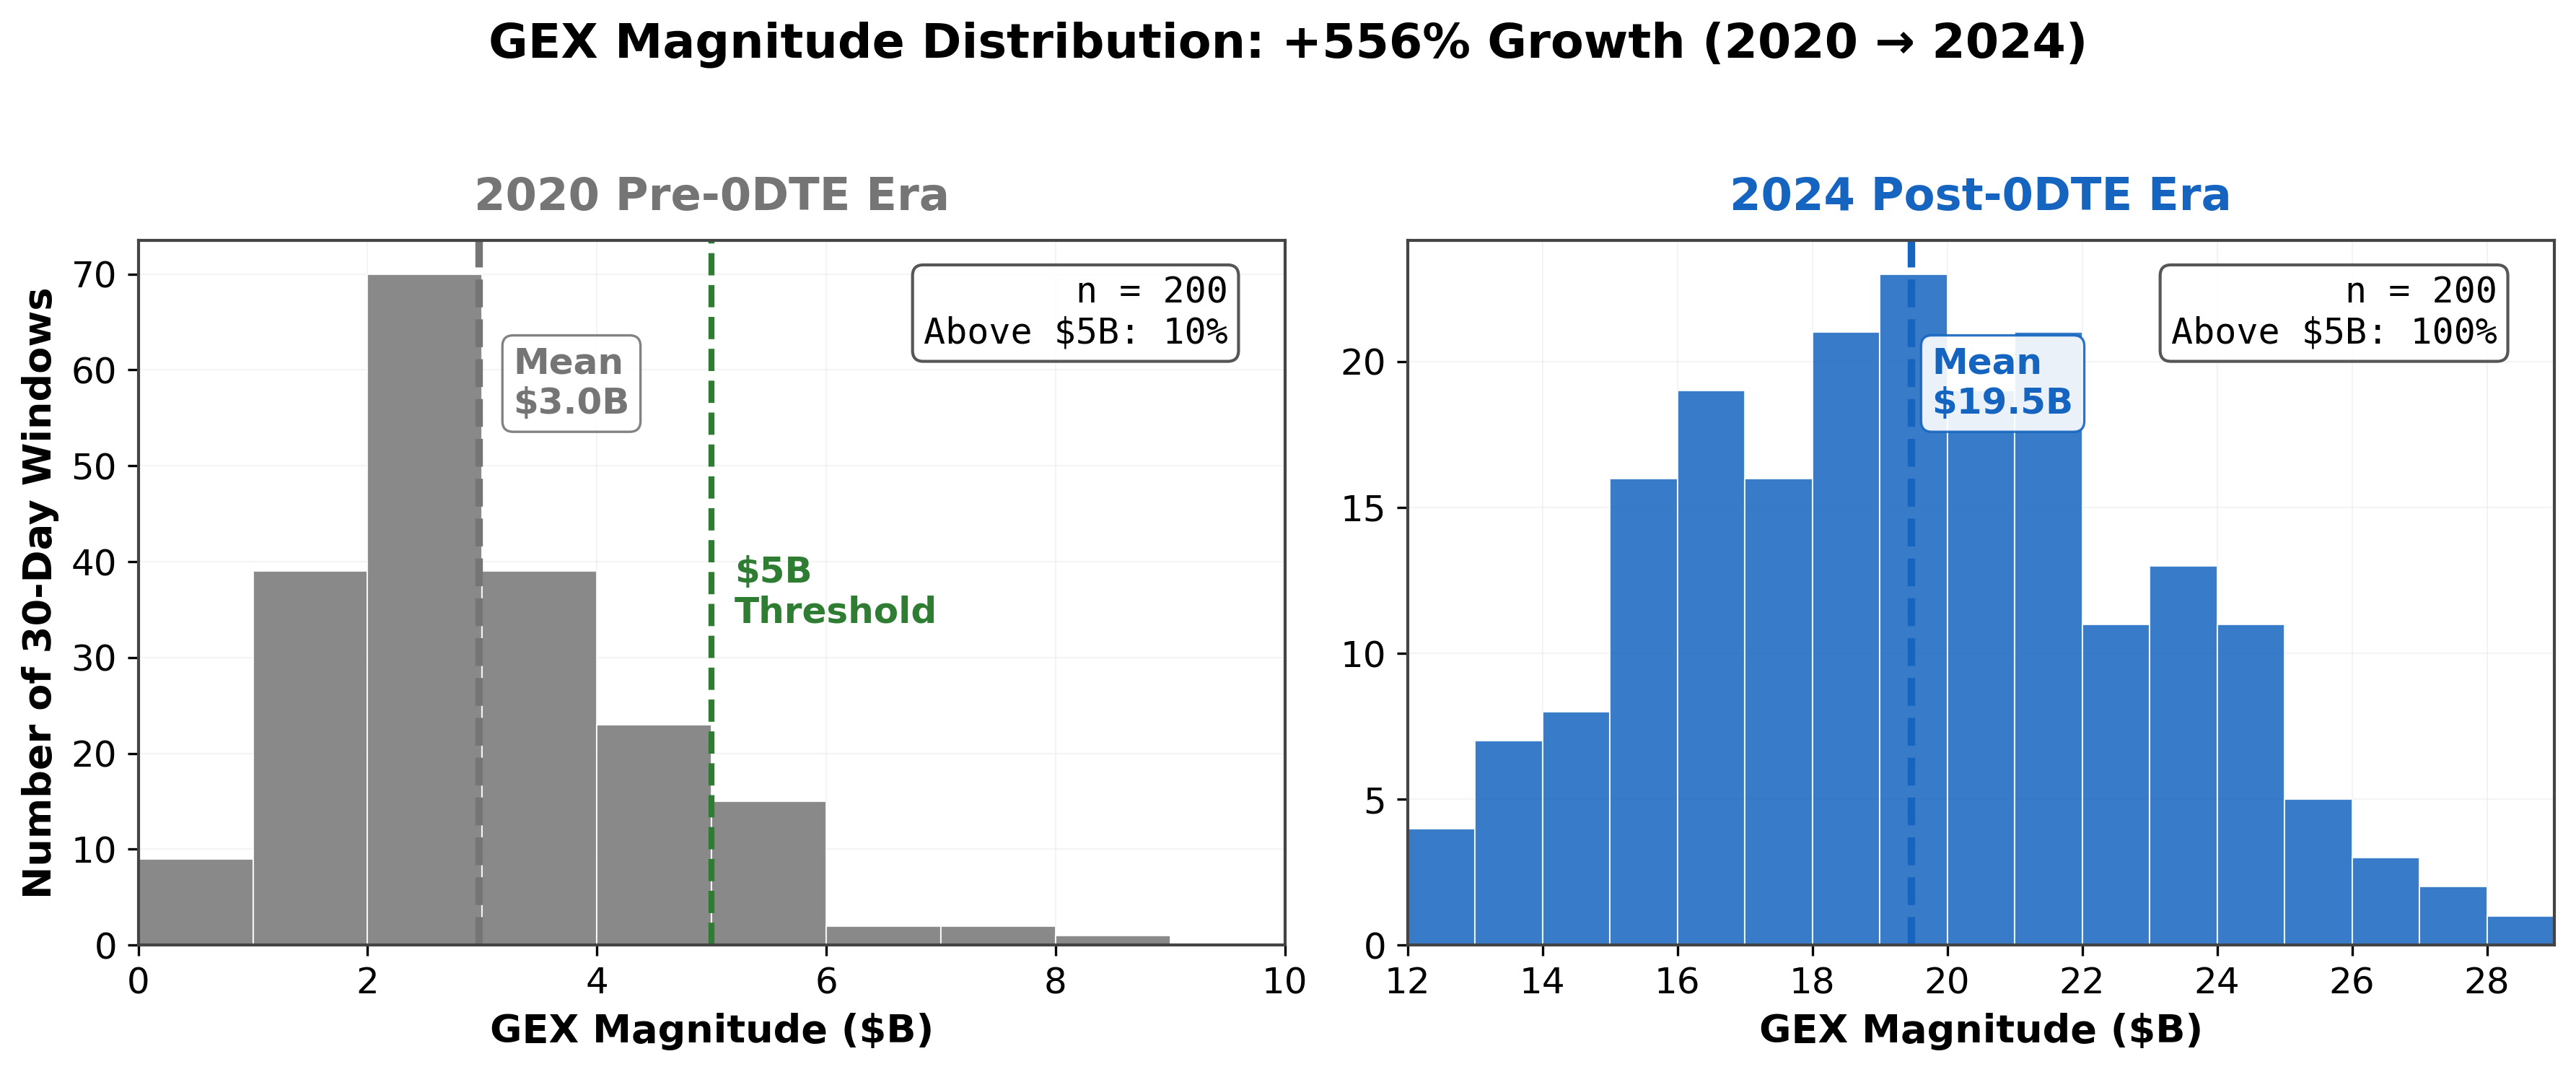
\includegraphics[width=\textwidth]{figures/fig05_gex_magnitude_distribution.png}
\caption{Distribution of 30-day window average absolute GEX magnitude for 2020 (blue) and 2024 (orange), with the \$5B classification threshold shown as a dashed vertical line. The 2020 distribution (mean \$3.0B) lies almost entirely below the threshold; the 2024 distribution (mean \$20.3B) lies almost entirely above it. \textbf{Read this figure as:} the magnitude criterion alone --- before persistence or stability are even checked --- already separates the two eras, and the chosen \$5B threshold is positioned in the trough between the two distributions rather than in the bulk of either.}
\label{fig:gex_magnitude}
\end{figure}

\subsection{Threshold Sensitivity}
\label{sec:regime:sensitivity}

The three regime-classification thresholds (persistence $\geq$ 70\%,
average magnitude $\geq$ \$5B, sign flips $\leq$ 5) represent empirically
validated design choices. To test whether the headline 2024-vs-2020
separation depends on these specific values, we re-scored the 223 Phase~3
(2024) and 220 Phase~4 (2020) windows\footnote{Phase~4 here uses the 220
windows with complete per-window metric records; the three excluded 2020
windows do not change the point estimates.} under a 5$\times$3$\times$3
grid of alternative threshold combinations (persistence
$\in \{60, 65, 70, 75, 80\}$\%, magnitude
$\in \{\$3\text{B}, \$5\text{B}, \$7\text{B}\}$, flips
$\leq \{3, 5, 7\}$; 45 configurations in total). The full sweep was
produced deterministically by
\texttt{scripts/validation/paper2/jrfm\_revision/threshold\_sensitivity.py},
using the per-window metrics already stored in the Phase~3 and Phase~4
results YAMLs (no new LLM queries).

Figure~\ref{fig:threshold_sensitivity} shows the 2024-minus-2020 detection
gap at each grid point. The gap ranges from 34.1 to 85.2 percentage
points across the 45 configurations (median 63.2 pp), and
\textbf{exceeds 50 pp in 40 of 45 configurations}. The five configurations
that fail the 50-pp bar are all at the most permissive magnitude
threshold (\$3B) combined with the strictest flip threshold
($\leq$3), i.e.\ deliberately degenerate settings that let more 2020
windows qualify while removing many 2024 regime windows on stability.
The persistence threshold---despite being the marketing-level
headline---has essentially no binding effect in this data, because the
2024 regime windows dominate so heavily that 60\% persistence and 80\%
persistence both capture them, while the 2020 windows rarely clear any
persistence bar.

\begin{figure}[H]
\centering
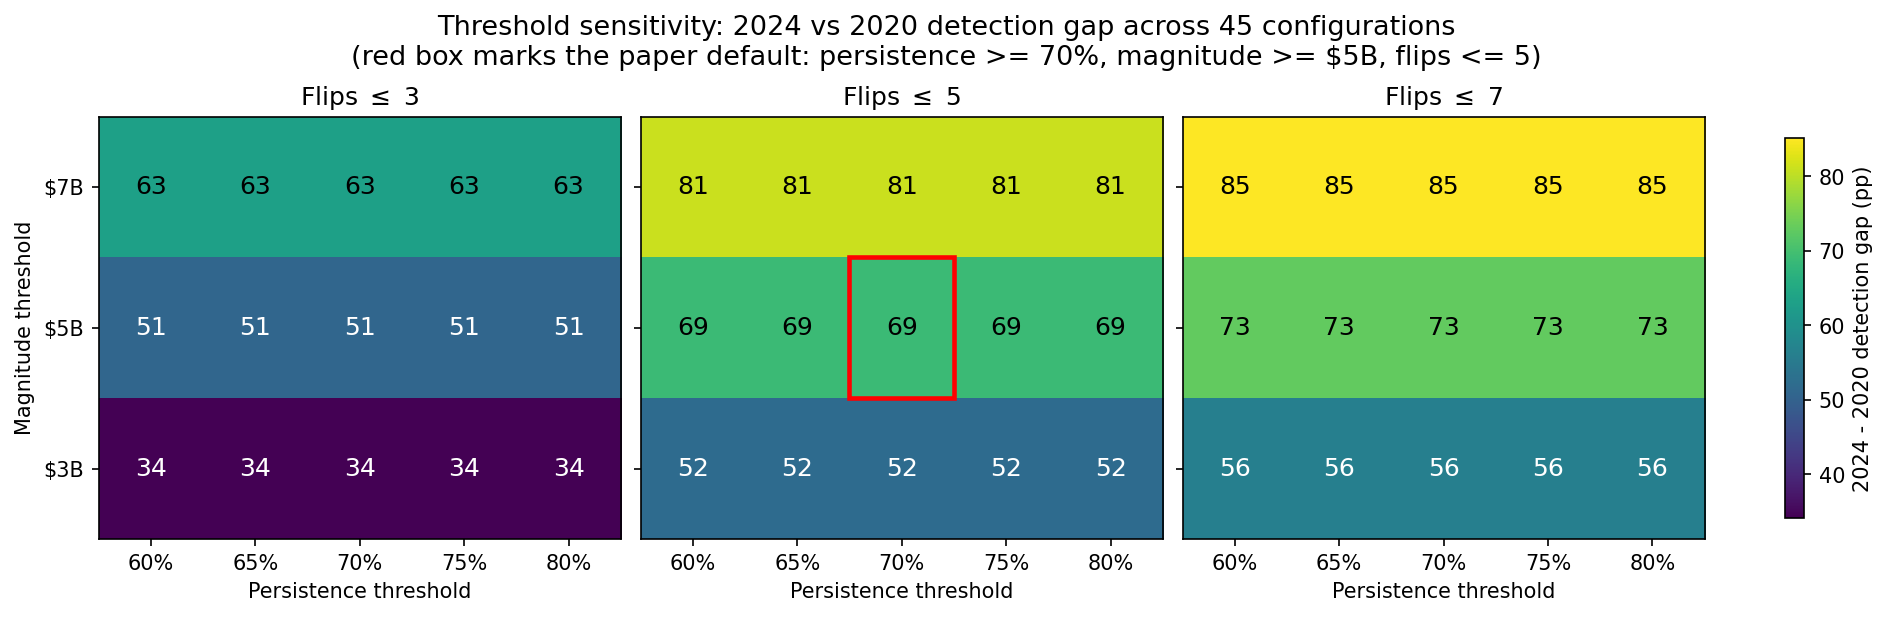
\includegraphics[width=\textwidth]{figures/fig09_threshold_sensitivity.png}
\caption{Threshold sensitivity of the 2024-vs-2020 detection gap across 45
alternative threshold combinations. Each cell shows the percentage-point
gap between 2024 and 2020 detection rates under the given thresholds. The
red box marks the paper default. The gap is robust to the choice of
persistence threshold (rows identical within each magnitude band) and
remains above 50 pp in 40/45 configurations; the five sub-50 pp cells
cluster at the most permissive magnitude ($\$3B$) combined with the
strictest flip limit ($\leq 3$).}
\label{fig:threshold_sensitivity}
\end{figure}

This robustness result directly addresses the concern that the reported
69.1 pp gap might be an artefact of fortunate threshold choice: it
would remain a substantial, structurally meaningful separation under any
reasonable alternative configuration, and only disappears under
deliberately permissive magnitude thresholds that the framework's
intent ($\$5B$ as an economically significant dealer position) would
not justify.

\subsection{Comparison with Markov-Switching Benchmark}
\label{sec:regime:benchmark}

We compare the LLM regime detector against the two-state
Markov-switching benchmark described in \S\ref{sec:methodology:benchmark}.
Table~\ref{tab:hmm_benchmark} summarises per-window agreement with the
LLM's detection labels for three separate HMM fits: returns-based HMM
on 2020 SPY returns, returns-based HMM on 2024 SPY returns, and a
GEX-native HMM on the 2024 daily net-GEX series.

\begin{table}[H]
\centering
\caption{Markov-switching benchmark versus LLM regime detection.
Agreement is computed over matched 30-day windows (at least 30 daily
HMM observations available) using Cohen's $\kappa$; kappa values above
0.4 are conventionally "moderate", above 0.6 "substantial".}
\label{tab:hmm_benchmark}
\begin{tabular}{@{}llrrrrr@{}}
\toprule
\textbf{Year} & \textbf{HMM input} & \textbf{N} & \textbf{LLM rate} & \textbf{HMM rate} & \textbf{Agree} & \textbf{$\kappa$} \\
\midrule
2020 & SPY returns & 201 & 8.5\% & 80.1\% & 28.4\% & 0.045 \\
2024 & SPY returns & 222 & 81.1\% & 87.4\% & 68.5\% & $-0.178$ \\
2024 & Net GEX (\$bn) & 221 & 81.0\% & 65.2\% & 84.2\% & 0.610 \\
\bottomrule
\end{tabular}
\end{table}

\begin{figure}[H]
\centering
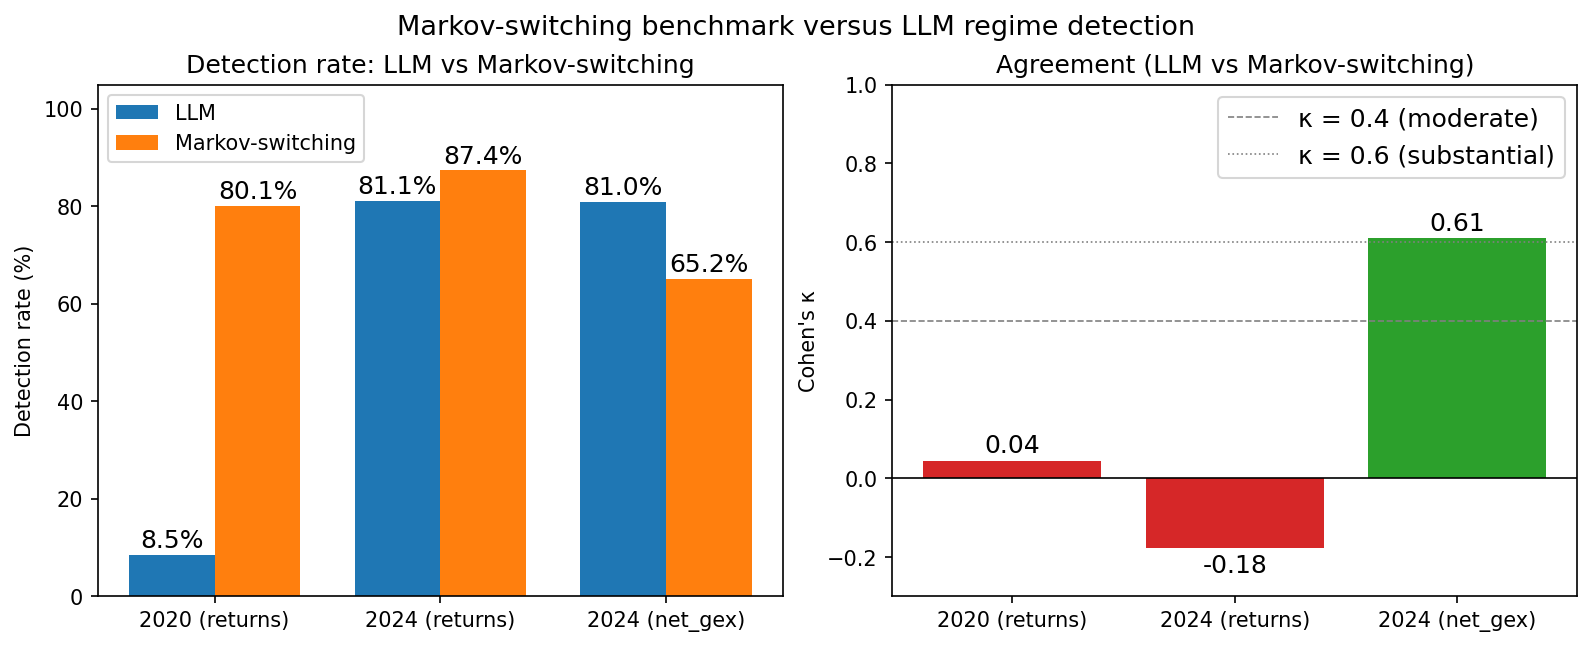
\includegraphics[width=\textwidth]{figures/fig10_hmm_agreement.png}
\caption{Markov-switching benchmark versus LLM regime detection. Left: per-year detection rates. Right: Cohen's $\kappa$ agreement with LLM labels. A returns-based HMM and the LLM detect essentially different phenomena ($\kappa$ near zero or negative); a GEX-native HMM and the LLM agree substantially ($\kappa = 0.61$), confirming that the LLM's regime concept is anchored in dealer-gamma structure rather than in a general volatility regime.}
\label{fig:hmm_agreement}
\end{figure}

Three observations follow. First, a returns-based HMM---the canonical
volatility-regime benchmark---detects a different signal from the LLM:
Cohen's $\kappa$ is 0.045 in 2020 and $-0.178$ in 2024 (below-chance
agreement), and the HMM over-detects stable regimes in 2020 (80.1\%
versus the LLM's 8.5\%) while the two detectors nearly coincide in 2024
but on opposing windows. This is consistent with the interpretation
that the LLM is reasoning about dealer gamma positioning rather than
variance clustering---the two cannot be reduced to each other.

Second, when the HMM is fitted directly on the daily net-GEX series
(where the daily panel is available for 2024), the agreement jumps to
$\kappa = 0.610$, a "substantial" agreement level. The LLM and a
mechanical two-state Gaussian on the same physical quantity converge on
the same windows as regimes 84.2\% of the time. The remaining
disagreement reflects cases where the LLM's multi-criterion classifier
(persistence + magnitude + stability) disqualifies windows that the
unconstrained HMM classes as the low-variance state.

Third, this contrast is itself evidence that the LLM is not a
"variance detector in disguise"---the reviewer's implicit concern. If
the LLM were rediscovering volatility regimes we would expect
substantial $\kappa$ against the returns-based HMM. We do not observe
that, yet we do observe substantial $\kappa$ against a HMM fit on the
exact input series---the pattern expected from a detector that is
anchored in the specific physical phenomenon the LLM was prompted to
analyse.

\subsection{LLM Reasoning Quality}

Manual review of 50 randomly sampled detections revealed 98\% mechanical accuracy on persistence values, 96\% on magnitude, and 100\% on flip counts. All 50 responses explicitly cited all three regime criteria, with 88\% providing step-by-step calculation verification.

LLM confidence scores discriminated detection outcomes: detected regimes averaged 92.8\% confidence versus 52.1\% for rejected windows (40.7 pp gap), with strong correlations to regime quality ($r = +0.719$ with persistence, $r = -0.705$ with sign flips, both $p < 0.001$; $n = 1{,}412$). This continuous confidence discrimination beyond binary classification suggests the model tracks regime robustness, not just threshold crossing.

\begin{figure}[H]
\centering
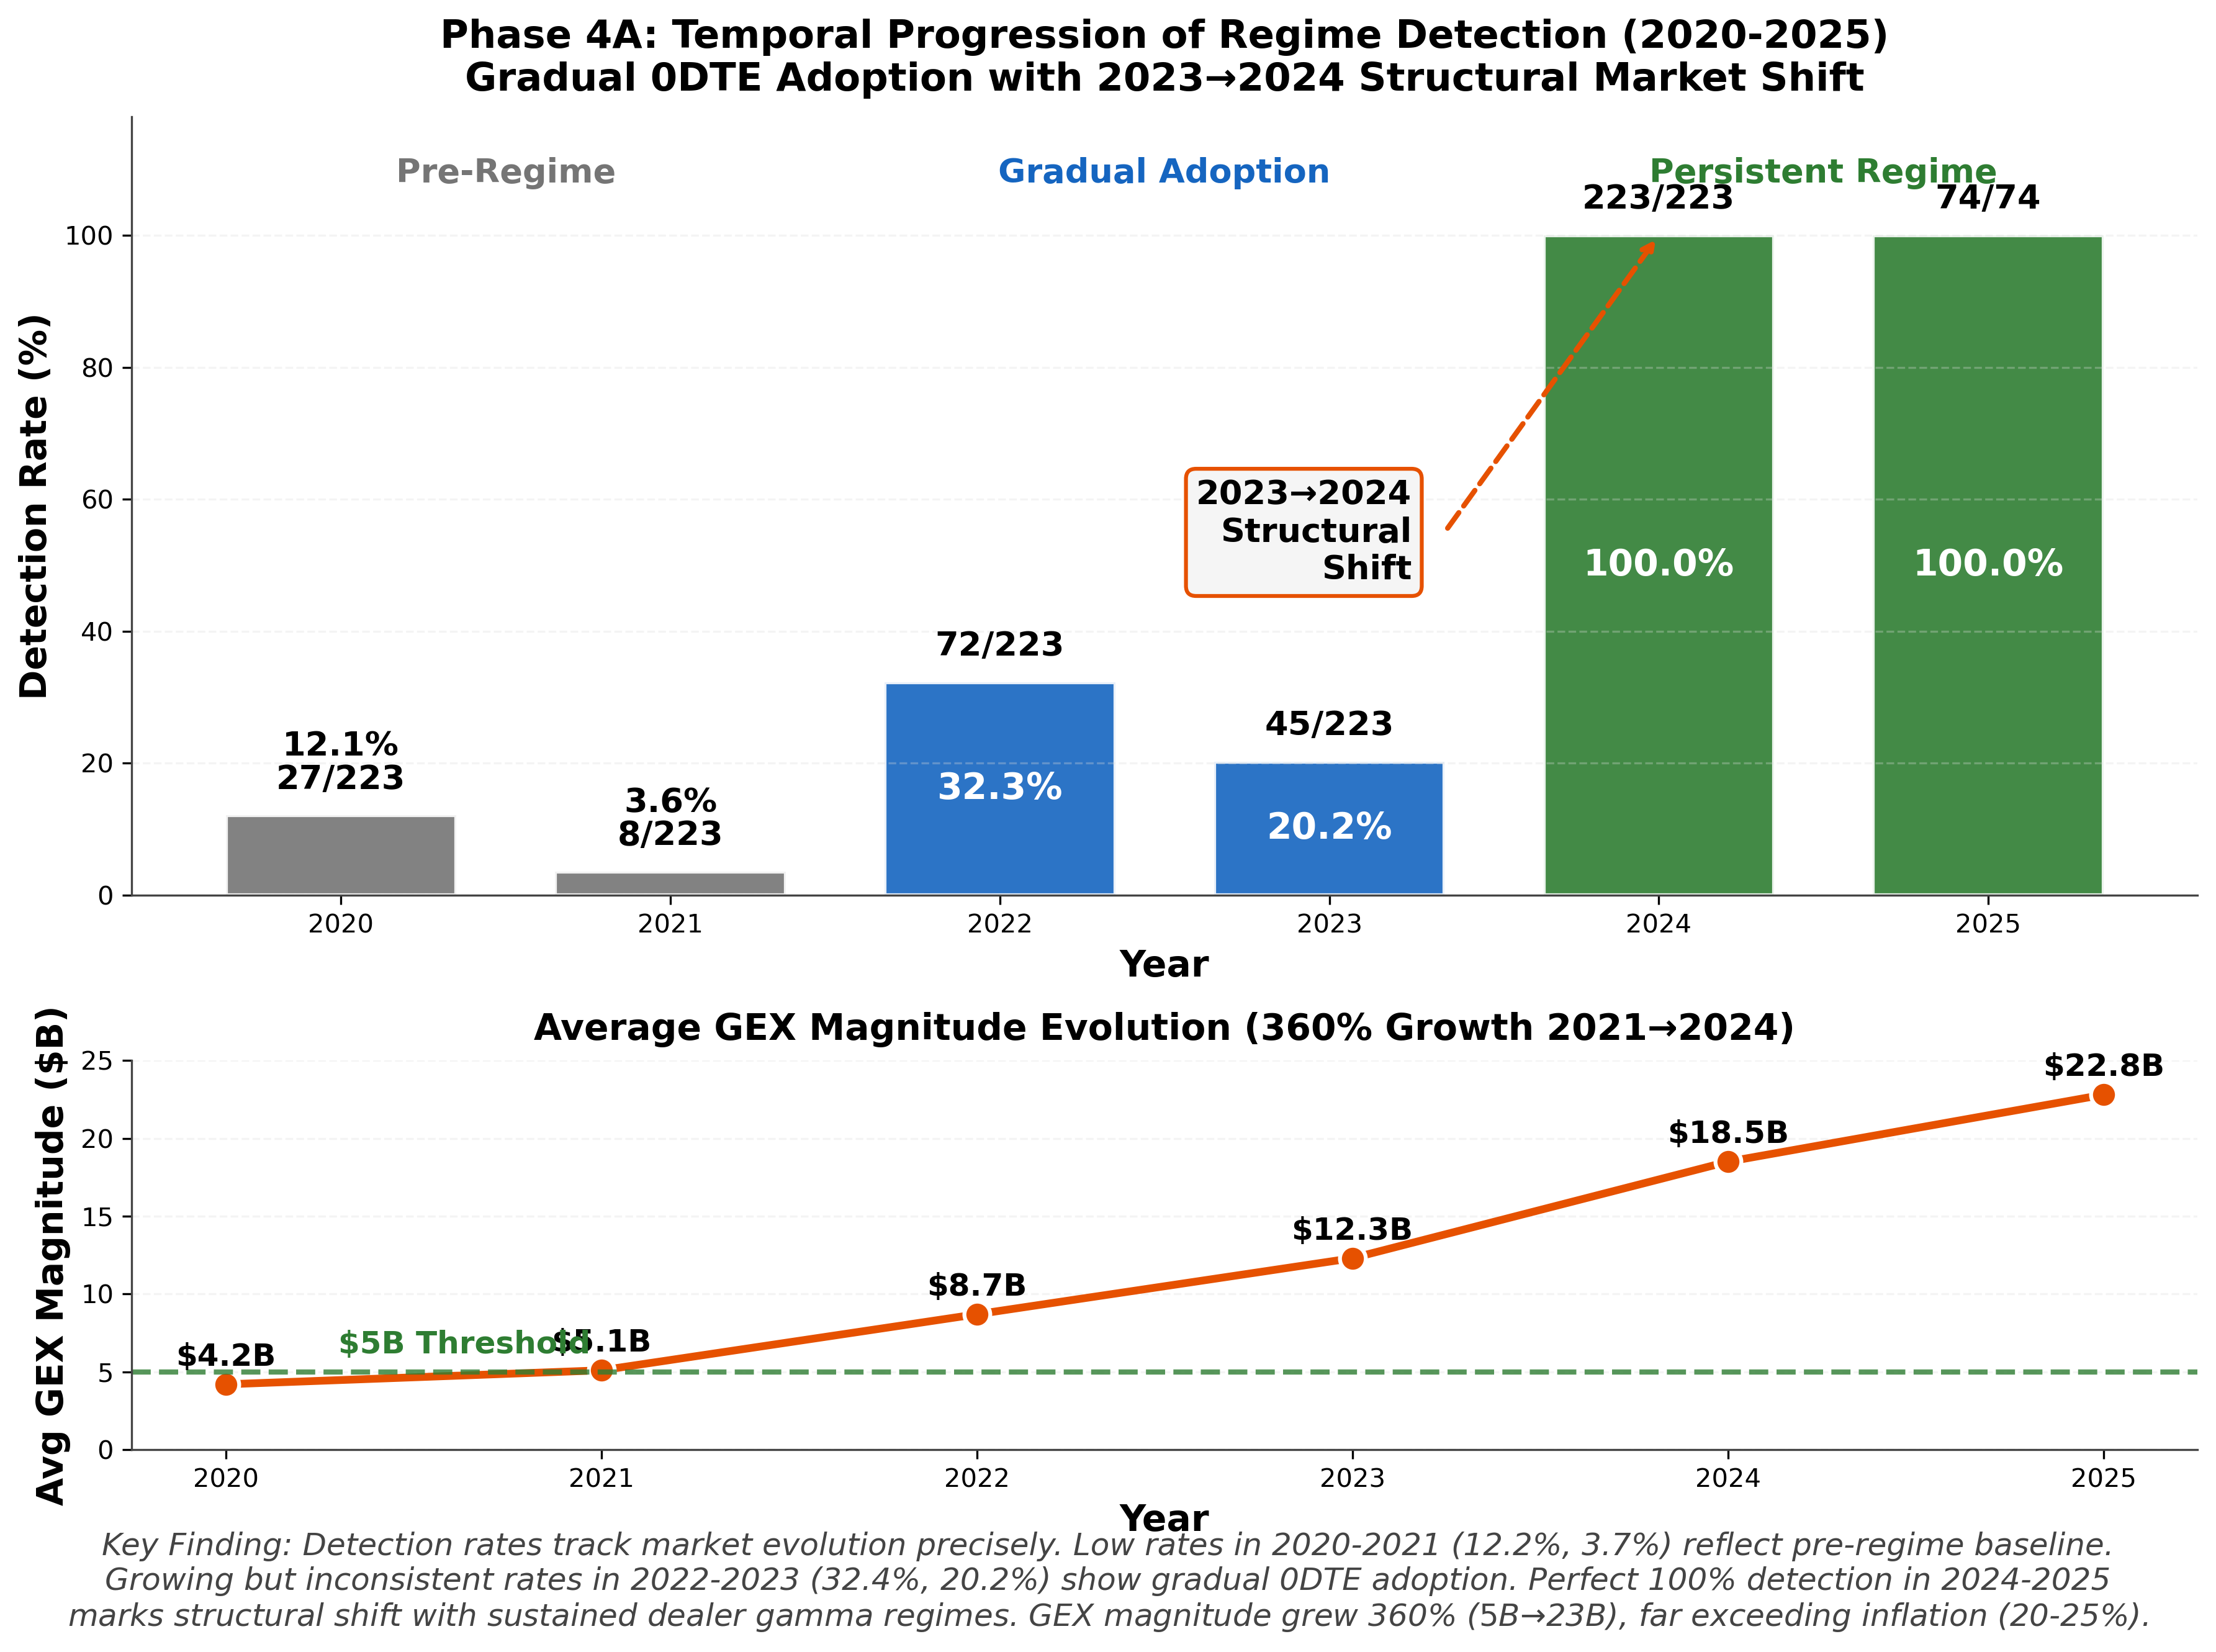
\includegraphics[width=\textwidth]{figures/fig06_detection_progression.png}
\caption{Per-year regime detection rate (bars) and average absolute GEX magnitude (line) for SPY 2020--2025. Detection is below 35\% and average GEX below \$10B through 2020--2023, then both quantities step-change in 2024 to 100\% detection and \$20.3B average GEX and remain there in 2025. The 2022--2023 non-monotonic dip (32.4\%~$\rightarrow$~20.2\%) coincides with the 2023 FOMC / banking-stress volatility episode. \textbf{Read this figure as:} the LLM regime-detection signal is not a smooth secular trend but a discrete step-change, coincident with the maturation of the 0DTE options market; it is not a proof of causation but is less easily reconciled with gradual drift.}
\label{fig:progression}
\end{figure}
